\documentclass[journal]{IEEEtran}

\usepackage{cite}
\usepackage{hyperref}
\usepackage{graphicx}

\usepackage{amsmath}
\interdisplaylinepenalty=2500

\usepackage{listings}
\lstset{basicstyle=\ttfamily\small, breaklines=true}

% correct bad hyphenation here
\hyphenation{op-tical net-works semi-conduc-tor}

\usepackage{xcolor}

\begin{document}

\title{Using fuzzy logic for extracting department and priority from email content}
\author{Peter Heemskerk, Stefan Schenk, Jim Kamans\\11988797, 11881798, 10302905}

% The paper headers
\markboth{Fuzzy Logic Email Classification}{}

\maketitle

% As a general rule, do not put math, special symbols or citations
% in the abstract or keywords.
\begin{abstract}
Large organizations often struggle to deliver emails or form emails to their corresponding departments if they are not directly addressed to a department or employee. Customer services are forced to read and forward the emails by hand, and cannot answer messages from external parties in a quick manner. This project aims to demonstrate that Fuzzy Logic can be used to solve this problem, by determining the correct department in an automatic way.

% These are general reasons for using Fuzzy Logic. Discuss why FL is useful for this specific problem.
\end{abstract}

\section{Introduction}
\IEEEPARstart{M}{any} large organizations suffer from their own complexity. If an external party seeks contact with a specific person in an organization, this usually works fine, but if a party seeks contact about a subject (without knowing whom to talk to), it usually takes more time before the party gets a good answer. At this moment emailing is the main way of communication to businesses, 120 billion email a year are sent which figure includes a large portion of spam mail \cite{email_statistics}.\\

%\subsection{Problem}

This project aims to solve this issue of customer service in a complex organization. We present software based on fuzzy logic which aims to bring a message of an external party to the correct internal department purely based on the content of the message.

One of the problems is that messages which would require attention of higher management are lost in the vast amount of received emails. Therefore a priority score is provided based on the email content.

%\subsection{Objectives}

The experiment has the goal to determine two outputs based on email content. First the correct department needs to be determined. Secondly a priority score. Based on the cleaned word lists a feature vector will be determined for each email. For department determination content specific features are uses. For priority determination two general features are designed.

For each email a feature vector is determined consisting of content and general features. These features are used as inputs in the fuzzy logic system to determine the two outputs: department and priority. \\

This project aims to prove that Fuzzy Logic works for this problem. Why fuzzy logic? Firstly, fuzzy logic deals well with incomplete or difficult to interpret data. Since there is a variety of email messages, short and long, specific and vague fuzzy logic better deals with these different sources. Secondly, fuzzy logic uses linguistic terms. With this we can include expert knowledge into the system which is relatively easy to interpret. This proves to be important for determining priority score from content, since no labeled data sets are available.\\

For our first goal department determination, our results can be compared to a given labeled data-set. Our second goal, using the same algorithms for determining a priority setting this experiment should be regarded as a proof-of-concept.

\section{Literature reviews}

Fuzzy Logic has been used earlier for email classification. Ferolin \cite{phishing}
has used fuzzy logic to implement a anti-phishing tool using content- and non-content eamil parameters. A RIPPER Classification Algorithm is used to learn relations of different phishing features, which translate into Fuzzy Logic rules. Santhi et al \cite{spam} determined the degree of dangerousness of spam email with a different method. A Fuzzy Logic system is used to categorize words that are spam in the degree to which these words are considered dangerous. The words are labeled to the names of five linguistic variables before they are fed to the particular input that corresponds with the name. Ferolin \cite{ranking} introduced a fuzzy logic based ranking function for efficient Information Retrieval. A fuzzy approach was used to rank words based on term-weighting schemes such as term frequency, inverse document frequency and normalization. The term frequency and inverse document frequency and normalization of the query and document are fed to their Fuzzy Logic Controller, whose outputs are fed to the main Fuzzy Logic Controller, which outputs a relevance score. None of these has utilized fuzzy logic for determining departments.

Douglass \cite{ranking} developed an email priority setting learning system for gmail based on social, content, search label features. These features are use in a statistical model which is parametrized for each user (recipiant) separately. This research does not present a solution for situations in larger organisations where there is no information about the individual recipient.

\section{Approach}
For email classification the following approach is followed. After data-preprocessing the email words are ranked, resulting in a feature score per email. Then fuzzy logic is applied to classify the email to the correct department and priority.

\subsection{Data}

A private dataset from ``Gemeente Amsterdam'' is used, containing 3589 emails with complaints from citizens.
This dataset is a csv file where each email has a correct department label, a description of the complaint, a description of contact with an employee and a proposed solution.
An example:
\begin{lstlisting}
Parkeren;Vrijdag voor een ...;Ja, contact
gezocht ...;De 23 euro ...
\end{lstlisting}

\subsection{Data preprocessing}
The data needs to be cleaned and filtered.

\begin{enumerate}
    \item Cleaning

    As an email body is read from the file system as plain text, individual terms are stored as individual values (``tokenized''). After that, capital characters are converted to lower case, punctuation and special characters are removed, stop-words are removed and the words are reduced to their base root form (``stemmed'').

    \item Filtering

    The remaining words may be meaningful now, but most of them may not be
    relevant. So the next operation will perform an intersection between the
    words and a list of predefined relevant words. All the words that reside
    in both lists will remain, but unlike sets, the list contains duplicates.
    As the last filtering step, the words are counted, and a corpus is created.

\end{enumerate}

\subsection{Ranking}

Other predefined sets of words within the set of relevant words share the
    same characteristics. For example a set $T \subseteq R$ exists where $T$
    is the set of technical words, and $R$ is the set of relevant words. Feature list of technical words: $T = [t_1, t_2, \dots, t_n]$.
    Other feature lists contain other themed words: $U$, $V$, $W$.

    For every word in the email that is present in $T$, a score is calculated
    that takes the count of that word into account in relation to the total
    number of relevant words in the email. This calculation is made for all
    feature lists ($T$, $U$, $V$, $W$), for every word in the email.

	For this experiment two types of features are chosen.
	The content type of feature determines the subject of the email, the second type are two general features: ``agitation'' which determines the negative emotion in an email, and ``action'' for addressing the neutral emergency of the email.

\subsection{Classification with Fuzzy Logic}

For determining the output variable department zeven content input variables are defined, corresponding with the content features. For determining the output variable priority two general input variables are defined, corresponding with the general features. Refer to \autoref{table:1}. For each of the input variables, 
three triangular membership functions (ms) are chosen to represent a low, medium or high value. For the output variable a triangular membership function is defined for each department. For the output variable priority, three membership functions have been defined: execution, management and political to represent the management-level on which the email needs to get attention to.  We have set a rule base for determining departments based on the content input variables and a rule base for determining priority based on the general input variables. An overview of the rules are in the attachment. \\

\begin{figure}
	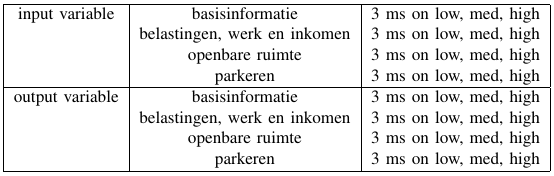
\includegraphics[scale=0.5]{res/inputs_outputs_FLS.png}
	\caption{Input and Output variables in Fuzzy Logic System}
	\label{table:1}
\end{figure}

%\begin{center}
%\begin{tabular}{ |c|c|c| }
% \hline
% input variable     & personal  & 3 ms on low, med, high    \\
% (content)          & tax       & 3 ms on low, med, high    \\
%                    & financial & 3 ms on low, med, high    \\
%                    & space     & 3 ms on low, med, high    \\
%                    & traffic   & 3 ms on low, med, high    \\
%                    & health    & 3 ms on low, med, high    \\
%                    & education & 3 ms on low, med, high    \\
% input variable     & agitation & 3 ms on low, med, high    \\
% (general)          & action    & 3 ms on low, med, high    \\
% output variable    & department & 5 ms for 5 departments   \\
% (content)          &           &                           \\
% output variable    & priority  & 3 ms on execution,        \\
% (general           &           & management, politics      \\
%
%\hline
%\end{tabular}
%\label{table:1}
%Input and Output variables in Fuzzy Logic System
%\end{center}

\subsection{Training and validation}

Our goal is two fold. Firstly, the use of fuzzy logic is tested to send an email to the right department. Secondly, with fuzzy logic we aim to solve how priority can be deducted from e-mail contents. The experimental approach for both is different.

\begin{enumerate}
    \item{Determining departments based on content}

    We can make this a supervised learning experiment, since we have for each email department labels available. We divide our data-set in a training set and validation set with factor 0.5. We train the system with the training set and validate on the validation set. Our feature lists (lists with trigger words for each content feature) is trained. For the Fuzzy Logic rule set we used our own expert knowledge.

    \item{Determining priority based on general features}

    To translate a received email based on its content to priority is more experimental and our data-set does not give labels for the outcome. The following approach is taken.

    For training the feature lists for input variables agitation and action 40 emails are randomly selected from our training-set and we have an independent experienced email reader score for these two input variables on a scale from 0 to 1. Based on these inputs, the feature lists are create resulting in the trigger words for agitation and for action.

    For validation we randomly selected 40 emails from our validation set and had an independent experienced email reader score for the output priority on a scale from 0 to 10. These values are used for validation.

\end{enumerate}

\subsection{Implementation}

For cooperation purposes we used Github \footnote{\url{https://github.com/Menziess/Fuzzy-Logic-Email-Classification}} (for source control) and Trello \footnote{\url{https://trello.com/fuzzylogicemailclassification}} (as scrum projectmanagement tool)

We used Python3 as programming language and Jupyter Notebook as development
environment. The code is enlisted in Attachment [ref]. For data-preprocessing Pythons NLTK module \footnote{\url{http://www.nltk.org/}} is used. For classification a new algorithm has been developed. The fuzzy logic system itself is based on the Fuzzy Logic LAB \footnote{\url{https://blackboard.uva.nl/webapps/blackboard/execute/content/file?cmd=view&content_id=_6947429_1&course_id=_212301_1&framesetWrapped=true}}, amended for using more than one output, a centroid defuzzifier and some more flexibility and error handling in management of fuzzy logic rules.

\section{Experiment}

\subsection{Results}

The automatic process of data-preprocessing, ranking and classification with fuzzy logic has been implemented. The systems works.

Validating the calculated departments with known labels has resulted in a low score.

Comparing the calculated priority with the score of the experience email reader is not fully implemented jet.

\subsection{Discussion}

Due to time-constraints the project has limitations: No references are found for the ranking part of the procedure and this part is therefore newly developed. The feature word list in this experiment has developed in a practical way, by combining training from known emails and adding words from different sources.

\section{Acknowledgment}

This work is done as part of the autumn 2017 bachelor course Fundamentals of Fuzzy Logic by A. Bilgin (and  M. Hol and V. Dankers) within the study Artificial Intelligence at University of Amsterdam.

\begin{thebibliography}{9}
\bibitem{email_statistics}
    The Radicati Group, inc.(2015),
    \textit{
        \href{https://github.com/Menziess/Fuzzy-Logic-Email-Classification/raw/master/report/res/a_new_fuzzy_logic_based_ranking_function_for_efficient_information_retrieval_system.pdf}{Email Statistics Report, 2015-2019},
    }.

\bibitem{spam}
    G.Santhi, S. Maria Wenish, Dr. P. Sengutuvan (2013),
    \textit{
        \href{https://github.com/Menziess/Fuzzy-Logic-Email-Classification/raw/master/report/res/a_content_based_classification_of_spam_mails_with_fuzzy_word_ranking.pdf}{A Content Based Classification of Spam Mails with Fuzzy Word Ranking},
    }
    Department of Information Science and Technology,
    Issue 3.

\bibitem{phishing}
    Rosana J. Ferolin, (2010 - approx.)
    \textit{
        \href{https://github.com/Menziess/Fuzzy-Logic-Email-Classification/raw/master/report/res/a_proactive_anti-phishing_tool_using_fuzzy_logic_and_ripper_data_mining_classification_algorithm.pdf}{A Proactive Anti-Phishing Tool Using Fuzzy Logic and RIPPER Data Mining Classification Algorithm},
    }
    Department of Computer Engineering University of San Carlos.

\bibitem{ranking}
    Rosana J. Ferolin, (2014)
    \textit{
        \href{https://github.com/Menziess/Fuzzy-Logic-Email-Classification/raw/master/report/res/a_new_fuzzy_logic_based_ranking_function_for_efficient_information_retrieval_system.pdf}{A new fuzzy logic based ranking function for efficient Information Retrieval system},
    }
    Department of Electrical Engineering Dayalbagh Educational Institute.

\bibitem{priority}
    Douglas Aberdeen, (2010 approx.)
    \textit{
        \href{[nog toevoegen}{The Learning behind Gmail Priority Inbox}
    }

\end{thebibliography}

\end{document}


